\subsection{Fine-Tuning Dynamics}
Fig.~\ref{fig:curves} shows the answer-token loss. Validation loss fell from 0.975 (base model, before any update) to 0.185 after one epoch; the training loss of the interrupted second epoch continued to decrease ($\approx$0.10), so the model had not yet converged when the run stopped. Because only the answer tokens are supervised and most of them are deterministic JSON syntax, a low loss is reached quickly; the remaining loss is concentrated in the label and evidence tokens, which is exactly where the model is weakest (below).

\begin{figure}[t]\centering
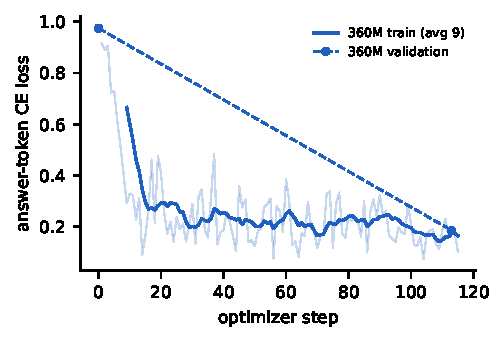
\includegraphics[width=\columnwidth]{figures/training_curves.pdf}
\caption{LoRA training of SmolLM2-360M: per-step training loss (light), 9-step moving average and validation loss after epoch 0 and 1. The run was terminated during epoch 2; the epoch-1 checkpoint is the final model.}\label{fig:curves}
\end{figure}

\subsection{Before vs.\ After Fine-Tuning and Label Strategies}
Table~\ref{tab:main} reports every model/strategy on the identical validation and test examples with identical greedy decoding. Three label strategies are compared on the \emph{same} forward passes: \emph{generated} (label parsed from the greedy JSON), \emph{scored} (argmax of the log-probability of each allowed label after the prompt) and \emph{calibrated} (scored plus per-type additive biases fitted on validation macro-F1 only and frozen for test).

\begin{table*}[t]\centering
\caption{Criterion-level results (greedy decoding, fp32, max.\ 48 new tokens; $n{=}206$ criteria per split). Accuracy (Acc), macro-F1 (mF1) overall and per criterion type; evidence micro-F1 over all records and macro-F1 over records with expert evidence; share of unparseable outputs (Inv.).}\label{tab:main}
\setlength{\tabcolsep}{4pt}
\begin{tabular}{lllrrrrrrrrr}\toprule
Split & Model & Label strategy & Acc & mF1 & Incl.\ Acc & Incl.\ mF1 & Excl.\ Acc & Excl.\ mF1 & Ev.\ micro-F1 & Ev.\ macro-F1 & Inv.\\\midrule
val & base & generated & 0.495 & 0.194 & 0.167 & 0.133 & 0.650 & 0.210 & 0.017 & 0.004 & 0.044 \\
val & base & scored & 0.592 & 0.232 & 0.318 & 0.138 & 0.721 & 0.210 & 0.017 & 0.004 & 0.000 \\
val & base & calibrated & 0.621 & 0.349 & 0.545 & 0.281 & 0.657 & 0.344 & 0.017 & 0.004 & 0.000 \\
val & LoRA & generated & 0.631 & 0.237 & 0.439 & 0.175 & 0.721 & 0.242 & 0.034 & 0.022 & 0.000 \\
val & LoRA & scored & 0.636 & 0.252 & 0.455 & 0.198 & 0.721 & 0.242 & 0.034 & 0.022 & 0.000 \\
val & LoRA & calibrated & 0.549 & 0.334 & 0.545 & 0.340 & 0.550 & 0.330 & 0.034 & 0.022 & 0.000 \\
\midrule
test & base & generated & 0.413 & 0.200 & 0.080 & 0.054 & 0.603 & 0.313 & 0.000 & 0.000 & 0.058 \\
test & base & scored & 0.519 & 0.263 & 0.213 & 0.124 & 0.695 & 0.273 & 0.000 & 0.000 & 0.000 \\
test & base & calibrated & 0.476 & 0.315 & 0.360 & 0.190 & 0.542 & 0.376 & 0.000 & 0.000 & 0.000 \\
test & LoRA & generated & 0.626 & 0.285 & 0.520 & 0.188 & 0.687 & 0.271 & 0.021 & 0.016 & 0.000 \\
test & LoRA & scored & 0.631 & 0.309 & 0.533 & 0.218 & 0.687 & 0.271 & 0.021 & 0.016 & 0.000 \\
test & LoRA & calibrated & 0.437 & 0.344 & 0.360 & 0.235 & 0.481 & 0.452 & 0.021 & 0.016 & 0.000 \\
\bottomrule\end{tabular}\end{table*}

\textbf{Effect of fine-tuning.} The base instruct model frequently ignores the schema, mixes the two label sets or answers in prose, which our parser maps to \emph{invalid} (Table~\ref{tab:main}, last column); the fine-tuned model produced valid JSON with an allowed label for every test record. On test, accuracy changes from \baseTestAcc{} to \ftTestAcc{} and macro-F1 from \baseTestFone{} to \ftTestFone{}. The gain in accuracy, however, mostly comes from learning the label \emph{priors}: the fine-tuned generator predicts ``not excluded'' for almost every exclusion criterion and ``not enough information'' for most inclusion criteria (Fig.~\ref{fig:cm}). Given 603 skewed training examples, one epoch and a 360M model, the cross-entropy objective is minimised well by the majority class---a classic imbalance failure that the mild class weighting ($w\propto f^{-1/2}$) did not overcome.

\textbf{Effect of the decision rule.} Scoring the allowed labels exposes the model's ranking, and calibration trades majority-class accuracy for minority-class recall: on test, the calibrated fine-tuned model reaches accuracy \calTestAcc{} and macro-F1 \calTestFone{}. Because biases were fitted on validation only, the test numbers are an honest estimate of this design choice; the remaining gap to useful performance shows that the representation, not just the decision threshold, is limiting. Calibration also helps the base model (test macro-F1 aseScTestFone{}$
ightarrow$0.315), and on the validation split---where the biases are fitted---the calibrated base model is even marginally ahead (0.349 vs.\ 0.334); on the held-out test split, however, the calibrated fine-tuned model is better (\calTestFone{} vs.\ 0.315), i.e.\ fine-tuning improves the label ranking that the decision rule exploits, but by a modest margin. We keep calibrated scoring as the default label strategy in the application (with the generated label shown alongside) and report all three.

\begin{figure*}[t]\centering
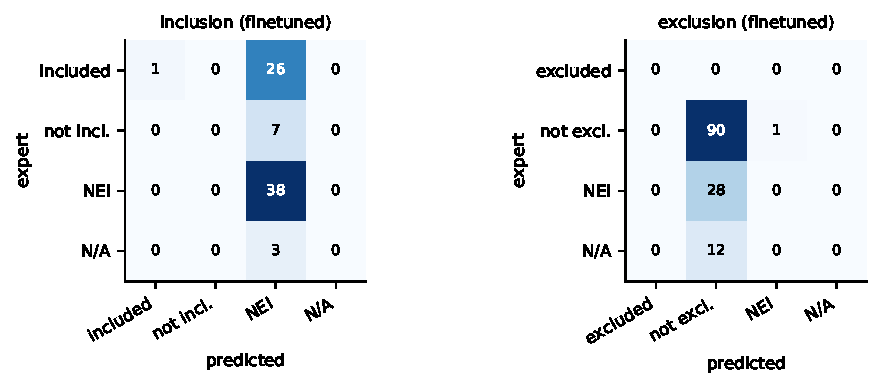
\includegraphics[width=0.49\textwidth]{figures/confusion_finetuned_test.pdf}\hfill
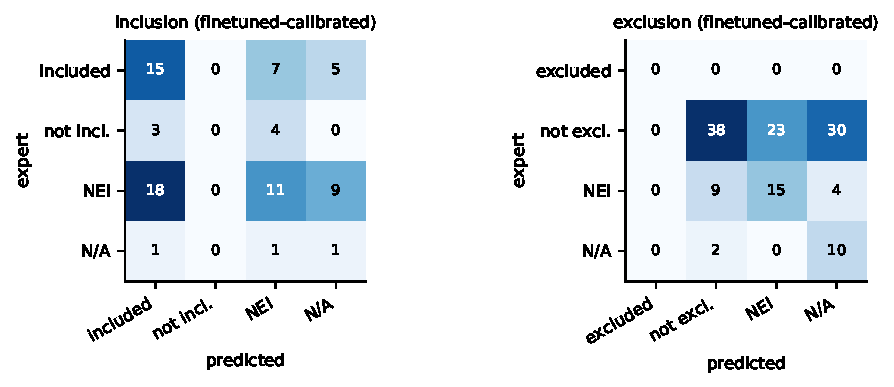
\includegraphics[width=0.49\textwidth]{figures/confusion_finetuned-calibrated_test.pdf}
\caption{Test confusion matrices for inclusion and exclusion criteria: fine-tuned model with generated labels (left pair) and with calibrated label scoring (right pair). NEI = not enough information, N/A = not applicable. The test split contains no ``excluded'' example.}\label{fig:cm}
\end{figure*}

\textbf{Per-class view.} Table~\ref{tab:perclass} lists precision, recall and F1 per class for the final configuration. Classes with fewer than five test examples (``not included'', ``not applicable'' for inclusion) are essentially unlearned; inclusion is harder than exclusion because the inclusion label distribution is not dominated by a single class.

\begin{table}[t]\centering\caption{Per-class test metrics, fine-tuned model with calibrated label scoring.}\label{tab:perclass}
\setlength{\tabcolsep}{3.5pt}
\begin{tabular}{llrrrr}\toprule
Type & Label & Supp. & P & R & F1\\\midrule
incl. & included & 27 & 0.405 & 0.556 & 0.469 \\
incl. & not included & 7 & 0.000 & 0.000 & 0.000 \\
incl. & not enough information & 38 & 0.478 & 0.289 & 0.361 \\
incl. & not applicable & 3 & 0.067 & 0.333 & 0.111 \\
excl. & excluded & 0 & 0.000 & 0.000 & 0.000 \\
excl. & not excluded & 91 & 0.776 & 0.418 & 0.543 \\
excl. & not enough information & 28 & 0.395 & 0.536 & 0.455 \\
excl. & not applicable & 12 & 0.227 & 0.833 & 0.357 \\
\bottomrule\end{tabular}\end{table}

\subsection{Evidence Sentence Localisation}
Table~\ref{tab:evidence} reports evidence retrieval on test. The fine-tuned model almost always outputs an empty evidence list: this gives perfect \emph{abstention accuracy} on the 60\% of records whose expert evidence is empty, but very low recall on records that do have evidence, hence a low micro-F1 (\ftTestEvF{}). The model never cited a non-existent sentence ID. This is the most important weakness of the system: the training target contains one or two evidence IDs for only 40\% of examples and the IDs are a small part of the loss, so the model learned that ``[]'' is the safest answer. Remedies within reach are evidence-only up-weighting of the ID tokens, a separate sentence-relevance scorer, or more epochs.

\begin{table}[t]\centering\caption{Evidence retrieval on test (fine-tuned, generated JSON). Micro over all records; macro over records with expert evidence ($n_{ev}$); abstention accuracy on records without expert evidence.}\label{tab:evidence}
\setlength{\tabcolsep}{3pt}
\begin{tabular}{lrrrrrrrr}\toprule
 & \multicolumn{3}{c}{Micro} & \multicolumn{3}{c}{Macro (gold$\neq\emptyset$)} & & \\
Subset & P & R & F1 & P & R & F1 & $n_{ev}$ & Abst.\\\midrule
overall & 1.000 & 0.011 & 0.021 & 0.016 & 0.016 & 0.016 & 61 & 1.000 \\
inclusion & 1.000 & 0.016 & 0.032 & 0.022 & 0.022 & 0.022 & 45 & 1.000 \\
exclusion & 0.000 & 0.000 & 0.000 & 0.000 & 0.000 & 0.000 & 16 & 1.000 \\
\bottomrule\end{tabular}\end{table}

\subsection{Error Analysis}
Of the 206 test criteria, the fine-tuned generator mislabels 77. Table~\ref{tab:errcats} groups all test records by error category (one record may fall in several) and Table~\ref{tab:errors} shows ten representative cases taken from \texttt{results/error\_analysis\_finetuned\_test.json}, each traceable to the original sentence IDs.

\begin{table}[t]\centering\caption{Error categories on test (fine-tuned, generated labels).}\label{tab:errcats}
\setlength{\tabcolsep}{3pt}
\begin{tabular}{lr}\toprule
Category & Records\\\midrule
Definite label with no cited sentence (unsupported decision) & 130\\
Gold definite $\rightarrow$ predicted ``not enough information'' (missed evidence) & 34\\
Gold ``not enough information'' $\rightarrow$ definite label (absence treated as proof) & 28\\
Correct label, evidence set differs from expert set & 27\\
Errors involving ``not applicable'' & 15\\
Hallucinated sentence IDs / invalid outputs & 0 / 0\\
\bottomrule\end{tabular}\end{table}

\begin{table*}[t]\centering\caption{Representative test errors of the fine-tuned model (patient sentence IDs in brackets). Gold/pred = expert/predicted label.}\label{tab:errors}
\footnotesize\setlength{\tabcolsep}{3pt}
\begin{tabular}{p{0.3cm}p{2.2cm}p{4.3cm}p{2.2cm}p{4.8cm}p{2.6cm}}\toprule
\# & Category & Criterion (type) & Gold $\rightarrow$ pred & Relevant patient evidence & Diagnosis\\\midrule
1 & missed evidence & Age greater than 18 years (incl.) & included $\rightarrow$ NEI & [0] ``\ldots a 67-year-old woman\ldots'' & explicit age not mapped to threshold\\
2 & missed evidence & Willing to give full informed consent (incl.) & included $\rightarrow$ NEI & [3] ``The patient will provide informed consent\ldots'' & near-verbatim match ignored\\
3 & absence as proof & Pre-operative eGFR $<$30 (excl.) & NEI $\rightarrow$ not excluded & none (no renal data) & majority prior for exclusions\\
4 & absence as proof & Previous axillary surgery (excl.) & NEI $\rightarrow$ not excluded & none & same; contradicts ``missing $\neq$ proof''\\
5 & not applicable & Pregnancy (excl.) & n/a $\rightarrow$ not excluded & [0] ``\ldots a 67-year-old woman\ldots'' (post-menopausal age) & applicability not reasoned\\
6 & not applicable & If female, using birth control (incl.) & n/a $\rightarrow$ NEI & [0] 15-year-old girl; [3] ``no sexual partners\ldots'' & conditional criterion\\
7 & unsupported (correct) & Prior central venous catheterisation (excl.) & not excl.\ $\rightarrow$ not excl. & [0] femoral arterial catheterisation & right label, no citation, wrong reason possible\\
8 & unsupported (correct) & Refused to sign informed consent (excl.) & not excl.\ $\rightarrow$ not excl. & [3] consent provided & right label, evidence omitted\\
9 & evidence only & Liver lesion requiring hepatic resection (incl.) & NEI $\rightarrow$ NEI & [3] ruptured liver abscess drained & related evidence not cited\\
10 & contradictory gold & Cautious selection, 5 types of liver damage (incl.) & NEI $\rightarrow$ NEI & [3] (expert cites a sentence yet labels NEI) & annotation itself partial\\
\bottomrule\end{tabular}\end{table*}

\textbf{Interpretation.} (i) The dominant failure is \emph{prior collapse}: 28 of the 77 label errors are ``not enough information'' exclusions labelled ``not excluded'' and 26 are ``included'' inclusions labelled ``not enough information''. These are opposite directions of the same behaviour---the model picks the type-specific majority class without reading the note---and cases 1--2 show that even trivially supported criteria (age, consent) are missed. (ii) Cases 3--4 are the safety-relevant direction: treating the absence of renal or surgical history as proof that an exclusion does not apply. Our pipeline does not hide this: because no sentence is cited, the explanation states that the decision rests on absence of evidence and the application lists such criteria under ``needs verification''. (iii) ``Not applicable'' requires conditional reasoning (sex-specific criteria, cases 5--6) that the model never learned from 28 training examples. (iv) Cases 7--10 have correct labels but missing evidence; case 10 is a contradictory annotation where the expert cites a sentence but still labels ``not enough information'', illustrating that evidence and label are not always aligned in the gold data. Calibrated scoring converts many type-(i) errors into minority predictions (higher macro-F1) but also introduces new false ``included''/``not applicable'' decisions, which is why its accuracy is lower (Table~\ref{tab:main}).


\subsection{KV-Cached Decoding}
Table~\ref{tab:kv} and Fig.~\ref{fig:kv} compare the uncached reference with the two cache implementations on the same fine-tuned model and the same real prompts (validation-split prompt tokens cut to the stated length), with EOS disabled so each run emits exactly the stated number of tokens (one warm-up, two timed runs, median reported).

\textbf{Token agreement.} For all four input/output settings with a reference (64/32, 256/32, 512/32, 128/64) the cached greedy tokens are \emph{identical} to the uncached ones, and the pre-allocated and concatenating caches agree with each other in all six settings. Unit tests extend this to three further lengths on the 135M model, to the tiled attention backend, to chunked prefill (a prompt fed in three pieces gives the same logits as one pass, $<10^{-4}$) and to cache cropping followed by re-feeding (the operation speculative decoding relies on). The benchmark logs the top-2 logit margin at the first divergent position if a mismatch occurs; none occurred, consistent with fp32 logit differences of $\sim10^{-5}$ being far smaller than typical greedy margins.

\begin{table*}[t]\centering\caption{KV-cache benchmark, fine-tuned SmolLM2-360M, fp32, 10 CPU threads. Times in seconds (median of 2 after warm-up); KV MB is the analytic fp32 cache size ($80$\,KiB/token); $\Delta$RSS is peak resident-memory increase (KV / no-cache).}\label{tab:kv}
\begin{tabular}{rrrrrrrrrrrl}\toprule
In & Out & No-cache & KV static & KV concat & KV prefill & KV decode & KV dec.\ tok/s & No-cache tok/s & KV MB & $\Delta$RSS MB & Same tokens\\\midrule
64 & 32 & 15.17 & 5.12 & 5.26 & 0.289 & 4.37 & 7.1 & 2.1 & 7.5 & 9/6 & yes \\
256 & 32 & 40.76 & 5.42 & 5.73 & 0.800 & 4.86 & 6.4 & 0.8 & 22.5 & 30/5 & yes \\
512 & 32 & 93.80 & 7.46 & 7.52 & 1.633 & 6.18 & 5.0 & 0.3 & 42.5 & 11/12 & yes \\
128 & 64 & 85.93 & 19.45 & 19.49 & 1.240 & 18.35 & 3.4 & 0.7 & 15.0 & 9/39 & yes \\
1024 & 64 & -- & 30.25 & 28.80 & 7.725 & 21.76 & 2.9 & -- & 85.0 & 761/-- & n/a \\
2048 & 32 & -- & 30.83 & 29.22 & 18.953 & 13.92 & 2.2 & -- & 162.5 & 97/-- & n/a \\
\bottomrule\end{tabular}\end{table*}

\begin{figure}[t]\centering
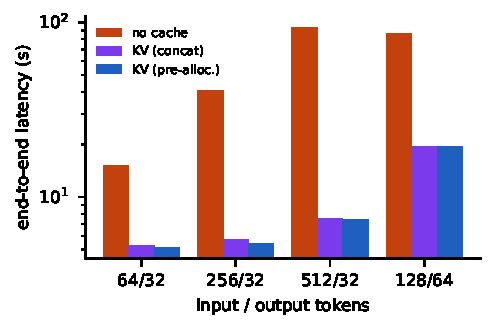
\includegraphics[width=\columnwidth]{figures/kv_latency.pdf}
\caption{End-to-end greedy generation latency (log scale) without cache, with a concatenating cache and with the pre-allocated cache.}\label{fig:kv}
\end{figure}

\textbf{Speed.} The cache turns each decode step from a forward pass over the whole sequence into a single-token pass, so the speed-up grows with context: 3.0$\times$ at 64 input tokens, 7.5$\times$ at 256 and \kvMaxSpeedup$\times$ at 512 (32 new tokens). Without a cache, throughput collapses from 2.1 to 0.34 tokens/s as the prompt grows; with the cache, decode throughput falls only mildly (7.1$\rightarrow$5.0 tokens/s) because attention over a longer cache is cheap compared to the weight-bound MLP and projection work. A single decode step must stream all 1.45\,GB of fp32 weights from memory, so 3--7 tokens/s is close to the memory-bandwidth limit of this laptop, which is why decode---not prefill---dominates end-to-end latency for short prompts. Prefill time scales roughly linearly to super-linearly with prompt length (0.29\,s for 64 tokens, 7.7\,s for 1{,}024, 19.0\,s for 2{,}048 tokens), reflecting the quadratic attention term at long contexts.

\textbf{Memory and cache growth.} The cache costs 80\,KiB per token (7.5\,MB at 96 tokens, 162\,MB at 2{,}080 tokens), small next to the 1.45\,GB of weights for our prompt lengths but linear in context and batch size, which is why GQA (5 instead of 15 KV heads, a 3$\times$ saving) matters. The measured RSS increases are dominated by allocator behaviour and transient activations (e.g.\ 761\,MB during the 1{,}024-token prefill) and are noisy; we report them but rely on the analytic sizes. The concatenating cache re-allocates every step ($O(N^2)$ copying) yet is within a few percent of the pre-allocated one at these lengths, because copying a few tens of MB is negligible next to a 1.45\,GB weight read; the pre-allocated cache's real advantage here is $O(1)$ roll-back for speculative decoding and a fixed memory footprint.


\subsection{Tiled Online-Softmax Attention}
\textbf{Correctness.} We compared all kernels with a float64 reference on eleven shapes covering single tokens ($T{=}S{=}1$), prefill ($T{=}S\in\{7,33,64,100,257,512,1024\}$), chunked prefill against a cache ($T{=}5,S{=}40$; $T{=}128,S{=}300$) and single-token decode against long caches ($T{=}1,S{=}129$), with $H{=}15$, $D{=}64$, batch 1--2 and the offset causal rule. Table~\ref{tab:attnerr} lists the worst-case and mean absolute errors. All fp32 variants and all tile sizes stay below $1.4\times10^{-6}$ and pass \texttt{allclose(atol=1e-5, rtol=1e-4)}; the float64 tiled kernel agrees to $4\times10^{-7}$ (limited by its fp32 inputs' rounding in the comparison). To stress the online softmax we multiplied the queries by 30 (logits in the hundreds): without max-subtraction $e^{s}$ would overflow, but both the explicit reference and the tiled kernel remain finite with the same $5\times10^{-5}$ error, which is the conditioning of the problem in fp32 rather than a kernel bug. Unit tests additionally check that perturbing future keys does not change earlier outputs (causality), and the whole decoder produces the same greedy tokens with \texttt{backend="tiled"} as with SDPA.

\begin{table}[t]\centering\caption{Attention numerical error vs.\ float64 reference (worst / mean over 11 shapes).}\label{tab:attnerr}
\begin{tabular}{lrr}\toprule
Implementation & Max $|\Delta|$ & Mean $|\Delta|$\\\midrule
reference\_fp32 & 1.4e-06 & 3.2e-08 \\
sdpa\_fp32 & 1.4e-06 & 3.1e-08 \\
tiled\_fp32\_b16x16 & 1.3e-06 & 2.9e-08 \\
tiled\_fp32\_b64x64 & 1.3e-06 & 3.0e-08 \\
tiled\_fp32\_b128x64 & 1.3e-06 & 3.0e-08 \\
tiled\_fp64\_b64x64 & 4.1e-07 & 1.2e-08 \\
tiled\_fp32\_b64x64\_scaled30 & 5.0e-05 & 2.9e-07 \\
reference\_fp32\_scaled30 & 5.0e-05 & 2.9e-07 \\
\bottomrule\end{tabular}\end{table}

\textbf{Speed and memory.} Fig.~\ref{fig:attn} and Table~\ref{tab:attnspeed} compare run time (median of 5 after warm-up). With small 64$\times$64 tiles the Python loop issues many tiny matrix products and is 2--4$\times$ \emph{slower} than the explicit reference, and 30$\times$ slower for single-token decode, where there is nothing to tile on the query side. Larger tiles amortise the interpreter overhead: with 256-wide tiles the tiled kernel is faster than the reference from $S{=}512$ on and, at $S{=}2048$, even faster than PyTorch's fused CPU SDPA (252 vs.\ 300\,ms), because it skips the $\approx$50\% of tiles above the causal diagonal while our SDPA call receives a dense boolean mask. The memory advantage is structural: the reference materialises fp32 score and probability matrices of $2HTS\cdot4$ bytes (480\,MB at $T{=}S{=}2048$), whereas the tiled kernel holds one tile (0.5--7.5\,MB). Measured RSS deltas are small and noisy for all kernels because PyTorch's CPU allocator reuses freed blocks between repetitions; we therefore report the analytic sizes as the reliable comparison. On GPUs a fused kernel such as FlashAttention also wins on speed because it keeps tiles in on-chip SRAM and fuses the exponentials and matrix products into one kernel launch; an educational PyTorch implementation cannot control memory placement, launches several operations per tile and runs the loop in Python, so it should not be expected to beat a fused kernel in general.

\begin{figure}[t]\centering
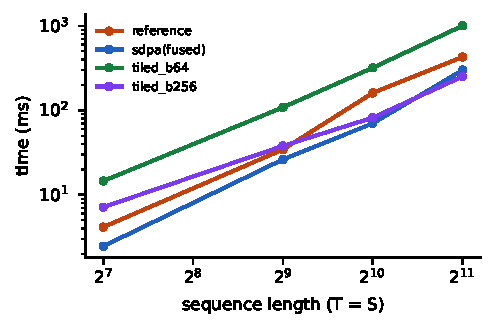
\includegraphics[width=\columnwidth]{figures/attn_speed.pdf}
\caption{Causal attention time for $T{=}S$ (15 heads, $D{=}64$, fp32, 10 CPU threads). Tiled performance depends strongly on tile size.}\label{fig:attn}
\end{figure}

\begin{table}[t]\centering\caption{Attention timing (ms, median of 5) and memory (peak RSS delta and analytic largest intermediate, MB).}\label{tab:attnspeed}
\setlength{\tabcolsep}{3pt}\footnotesize
\begin{tabular}{rrlrrr}\toprule
$T$ & $S$ & Impl. & ms & $\Delta$RSS & Interm.\\\midrule
128 & 128 & reference & 4.14 & 0.4 & 1.88 \\
128 & 128 & sdpa(fused) & 2.46 & 0.1 & fused \\
128 & 128 & tiled\_b64 & 14.56 & 0.1 & 0.47 \\
128 & 128 & tiled\_b128 & 6.90 & 1.0 & 1.88 \\
128 & 128 & tiled\_b256 & 7.14 & 1.0 & 1.88 \\
512 & 512 & reference & 34.40 & 4.0 & 30.00 \\
512 & 512 & sdpa(fused) & 26.22 & 0.1 & fused \\
512 & 512 & tiled\_b64 & 108.49 & 0.0 & 0.47 \\
512 & 512 & tiled\_b128 & 57.84 & 0.0 & 1.88 \\
512 & 512 & tiled\_b256 & 37.91 & 0.0 & 7.50 \\
1024 & 1024 & reference & 160.77 & 0.0 & 120.00 \\
1024 & 1024 & sdpa(fused) & 70.10 & 5.7 & fused \\
1024 & 1024 & tiled\_b64 & 319.28 & 3.8 & 0.47 \\
1024 & 1024 & tiled\_b128 & 133.62 & 0.8 & 1.88 \\
1024 & 1024 & tiled\_b256 & 81.88 & 0.0 & 7.50 \\
2048 & 2048 & reference & 428.78 & 0.0 & 480.00 \\
2048 & 2048 & sdpa(fused) & 299.58 & 5.7 & fused \\
2048 & 2048 & tiled\_b64 & 1003.66 & 8.0 & 0.47 \\
2048 & 2048 & tiled\_b128 & 395.49 & 0.0 & 1.88 \\
2048 & 2048 & tiled\_b256 & 251.57 & 0.1 & 7.50 \\
1 & 1024 & reference & 2.06 & 0.0 & 0.12 \\
1 & 1024 & sdpa(fused) & 0.84 & 0.0 & fused \\
1 & 1024 & tiled\_b64 & 27.13 & 0.0 & 0.01 \\
1 & 1024 & tiled\_b128 & 9.53 & 0.0 & 0.01 \\
1 & 1024 & tiled\_b256 & 8.18 & 0.0 & 0.03 \\
1 & 4096 & reference & 4.65 & 0.0 & 0.47 \\
1 & 4096 & sdpa(fused) & 1.24 & 0.1 & fused \\
1 & 4096 & tiled\_b64 & 30.58 & 0.0 & 0.01 \\
1 & 4096 & tiled\_b128 & 20.82 & 0.0 & 0.01 \\
1 & 4096 & tiled\_b256 & 11.44 & 0.0 & 0.03 \\
64 & 2048 & reference & 11.55 & 0.0 & 15.00 \\
64 & 2048 & sdpa(fused) & 11.90 & 0.0 & fused \\
64 & 2048 & tiled\_b64 & 33.85 & 0.0 & 0.47 \\
64 & 2048 & tiled\_b128 & 29.43 & 0.0 & 0.94 \\
64 & 2048 & tiled\_b256 & 19.20 & 0.0 & 1.88 \\
\bottomrule\end{tabular}\end{table}


\subsection{Speculative Decoding}
Table~\ref{tab:spec} and Fig.~\ref{fig:specfig} compare speculative decoding with ordinary KV-cached greedy decoding of the same fine-tuned target on three validation prompts (different patients), for two workloads: \emph{task} (the real screening prompt; the JSON answer has 14 tokens and stops at \texttt{<|im\_end|>}) and \emph{long} (EOS disabled, 64 new tokens). The draft is the base SmolLM2-135M-Instruct; $k\in\{1,2,4\}$; one warm-up and two timed runs per configuration.

\textbf{Correctness.} All 18 speculative runs produced exactly the same token sequence as greedy decoding of the target, for every $k$; unit tests add three more $k$ values and a self-drafting test (target used as its own draft) in which, as expected, every drafted token is accepted. The invariant-based cache handling---cropping the target cache to the committed prefix after each verification and letting the draft cache lag by at most one token---is what makes this exact. As an external reference we also ran Hugging Face assisted generation with the same models; it stopped after 5 tokens whereas our greedy and speculative decoders produced the full 14-token answer, so this cross-check was inconclusive (most likely a difference in how the merged LoRA weights or the stop token were passed to the library) and we rely on equality with our own verified greedy path instead.

\begin{table}[t]\centering\caption{Speculative vs.\ greedy decoding (target: fine-tuned SmolLM2-360M; draft: SmolLM2-135M). Acc.\ = accepted/drafted tokens; tok/pass = committed tokens per target forward; speed-up = greedy latency / speculative latency (mean over prompts).}\label{tab:spec}
\setlength{\tabcolsep}{3pt}
\begin{tabular}{lcccccc}\toprule
Draft & $k$ & Same & Acc. & tok/pass & tok/s & Speed-up\\\midrule
\multicolumn{7}{l}{\textit{task workload} (3 prompts, mean new tokens 14; greedy 3.1 tok/s)} \\
base\_135m & 1 & yes & 0.625 & 1.56 & 2.5 & 0.76 \\
base\_135m & 2 & yes & 0.667 & 2.00 & 3.5 & 1.14 \\
base\_135m & 4 & yes & 0.364 & 2.00 & 2.4 & 0.79 \\
\multicolumn{7}{l}{\textit{long workload} (3 prompts, mean new tokens 64; greedy 3.8 tok/s)} \\
base\_135m & 1 & yes & 0.863 & 1.83 & 4.6 & 1.24 \\
base\_135m & 2 & yes & 0.825 & 2.57 & 4.7 & 1.25 \\
base\_135m & 4 & yes & 0.690 & 3.53 & 5.1 & 1.38 \\
\bottomrule\end{tabular}\end{table}

\begin{figure}[t]\centering
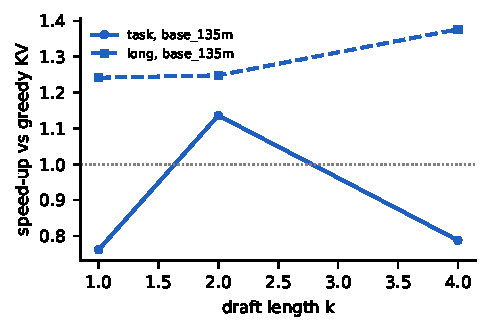
\includegraphics[width=\columnwidth]{figures/spec_speedup.pdf}
\caption{Mean speed-up of speculative over greedy decoding as a function of draft length $k$ for the short task answers and 64-token generation.}\label{fig:specfig}
\end{figure}

\textbf{Efficiency.} On long generation the draft agrees with the target on 86\% of drafted tokens at $k{=}1$ and 69\% at $k{=}4$, so each target pass commits 1.8--3.5 tokens and speculative decoding is 1.24--1.38$\times$ faster on average (up to 1.63$\times$ on one prompt). On the short task answers it is mostly \emph{slower} (0.76$\times$ at $k{=}1$, 0.79$\times$ at $k{=}4$; only $k{=}2$ gains, 1.14$\times$). Three effects explain this. (i) The cost ratio is unfavourable: a decode step of either model is memory-bandwidth bound, so the 135M draft costs roughly its share of weight bytes, $pprox$37\% of a 360M target pass (0.54 vs.\ 1.45\,GB), whereas the expected speed-up of speculative decoding grows as the draft-to-target cost ratio shrinks~\cite{leviathan2023fast}. (ii) With only 14 output tokens, the fixed costs---prefilling the draft as well as the target, and the first token that must come from the target---are amortised over very few tokens. (iii) The base draft was not fine-tuned, so it disagrees with the fine-tuned target exactly on the informative label tokens (acceptance 36\% at $k{=}4$ on the task workload); a longer $k$ then wastes draft passes on rejected tokens. Memory overhead is the second model (0.54\,GB fp32) plus its cache (45\,KiB/token). A fine-tuned draft, smaller drafts (e.g.\ layer-skipping self-speculation) or batch serving on a GPU, where the target pass is compute-light relative to its fixed overhead, are the natural ways to turn the measured acceptance into speed.


\subsection{Application}
Fig.~\ref{fig:app} shows the screening view on an unseen, hand-written patient note (62-year-old man with type 2 diabetes, HbA1c 9.1\%, eGFR 48, myocardial infarction two years ago). With calibrated label scoring the three inclusion criteria are judged ``included'', pregnancy ``not applicable'', and pancreatitis and recent infarction ``not excluded''; the eGFR$<$30 exclusion is judged ``not enough information'' although sentence 3 states an eGFR of 48---a missed-evidence error of the kind analysed above. The generated JSON alone would have answered ``not enough information'' for all inclusions, illustrating the prior collapse. Because no sentence is cited, every definite decision is listed for human verification. Each criterion card shows the label, the cited sentences (highlighted in the record panel when the card is clicked), the explanation and timing; the summary card shows the rule-based outcome with the blocking, missing-information and needs-verification lists. Invalid inputs (empty note, malformed NCT ID, $>$40 criteria, model still loading) return readable messages without losing the user's input, and every run is persisted as JSON and downloadable as an HTML report with provenance.

\begin{figure}[t]\centering
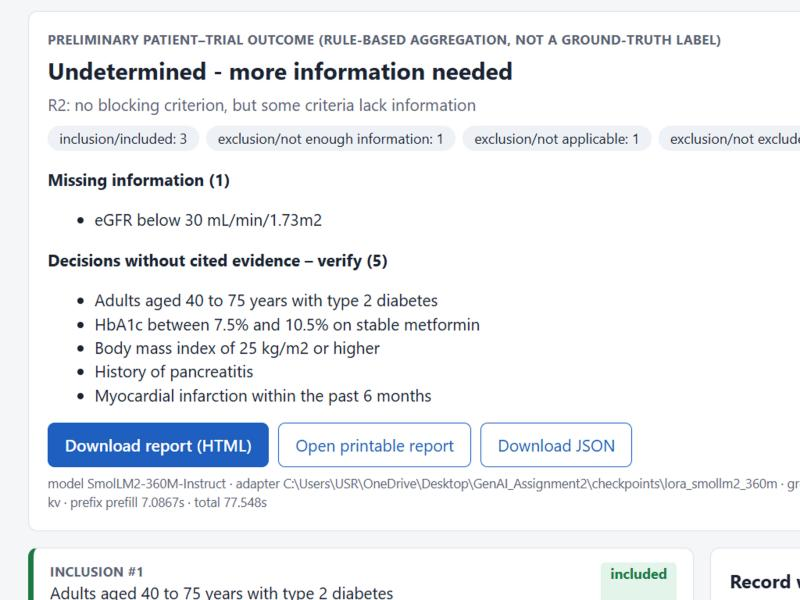
\includegraphics[width=0.49\columnwidth]{figures/app_screen.jpg}\hfill
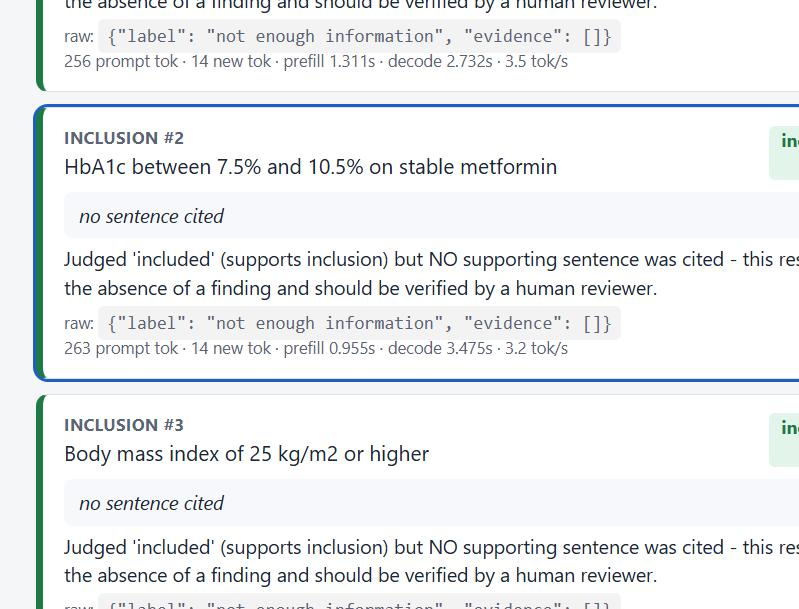
\includegraphics[width=0.49\columnwidth]{figures/app_cards.jpg}
\caption{TrialMatch-Lite on the unseen hand-written case. Left: rule-based preliminary outcome with the missing-information and needs-verification lists, report export buttons and provenance. Right: criterion cards with label, cited evidence (none here), explanation that flags the absence of evidence, raw model output and timing.}\label{fig:app}
\end{figure}
